\documentclass[eikonal.tex]{subfiles}

\begin{document}

\section{Introduction}\label{sec:introduction}

We develop fast, memory efficient, and accurate solvers for the
eikonal equation, a nonlinear hyperbolic PDE encountered in
high-frequency wave propagation~\cite{engquist2003computational} and
the modeling of a wide variety of problems in computational and
applied science~\cite{sethian1999level}, such as photorealistic
rendering~\cite{ihrke2007eikonal}, constructing signed distance
functions in the level set method~\cite{osher2006level}, solving the
shape from shading
problem~\cite{kimmel2001optimal,prados2006shape,durou2008numerical},
traveltime computations in numerical modeling of seismic wave
propagation~\cite{sethian19993,popovici20023,kim20023,van1991upwind,vidale1990finite},
and others. We are motivated primarily by problems in high-frequency
acoustics~\cite{prislan2016ray}, which are key to enabling a higher
degree of verisimilitude in virtual reality simulations
(see~\cite{raghuvanshi2014parametric,raghuvanshi2018parametric} for a
cutting-edge time-domain approach which is useful up to moderate
frequencies). Current approaches to acoustics simulations rely on
methods whose complexity depends on the highest frequency of the sound
being simulated. For moderately high-frequency wave propagation
problems, the eikonal equation comes about as the first term in an
asymptotic WKB expansion of the Helmholtz equation and corresponds to
the first arrival time of rays propagating under geometric optics,
although approaches for computing multiple arrivals
exist~\cite{fomel2002fast}.

In this work, we develop direct solvers for the eikonal equation which
are fast and accurate, particularly in 3D. We develop two separate
families of algorithms which approach the problem of efficiently
computing updates in 3D in separate ways. These algorithms are
analyzed and extensive numerical studies are carried out. Both
approaches use knowledge of the problem gleaned from its Lagrangian
representation to reduce the amount of computational work necessary to
compute an accurate result. These approaches are competitive with
existing direct solvers for the eikonal equation and readily
generalize to related equations (the static Hamilton-Jacobi equation)
and higher dimensions. This research was conducted in tandem with
research into ordered line integral methods for computing the
quasipotential of nongradient stochastic differential equations
(SDEs)~\cite{dahiya2017ordered,dahiya2018ordered,yang2019computing};
however, because of the comparative simplicity of the eikonal
equation, we were led to develop two separate families of algorithms
(one based on the original quasipotential ordered line integral
method, but modified) that were more amenable to analysis, which
allowed us to obtain theoretical results that justify our experimental
findings.

\subsection{Results}

\begin{figure}
  \centering
  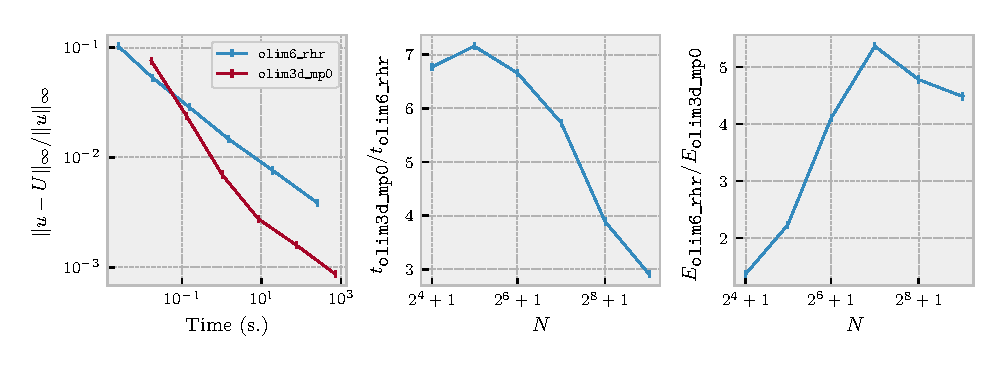
\includegraphics[width=\linewidth]{intro.eps}
  \vspace{-2em}
  \caption{\emph{Comparing \texttt{olim3d\_mp0} and
      \texttt{olim6\_rhr}.} For the multiple point source problem in
    \cref{ssec:slotnick} with the domain $\Omega = [0, 1]^3$
    discretized in each direction into $N = 2^p + 1$ (where
    $p = 4, 5, \hdots, 9$); the total number of grid points is
    $N^3$. The plots show from left to right: 1) the relative
    $\ell_\infty$ error plotted vs.\ CPU runtime in seconds, 2)
    quotient of CPU times, 3) quotient of $\ell_\infty$
    errors.}\label{fig:intro}
\end{figure}

Different numerical methods have been proposed for the solution of the
eikonal equation; generally, there are direct solvers and iterative
solvers. The most popular direct solvers are based on Dijkstra's
algorithm (we refer to these as ``Dijkstra-like'' from now
on)~\cite{tsitsiklis1995efficient,sethian1996fast}, and the most
popular iterative method is the fast sweeping
method~\cite{tsai2003fast,zhao2005fast}. In this work, we develop a
family of Dijkstra-like solvers for the eikonal equation in 2D and 3D,
similar to the fast marching method (FMM) or ordered upwind
methods~\cite{sethian1996fast,sethian2003ordered}. These solvers come
about by discretizing and minimizing the action functional for the
eikonal equation (see \cref{sec:minimum-action-integral}). We
investigate three different quadrature rules for discretizing this
line integral: a righthand rule (\texttt{rhr}), a simplified midpoint
rule (\texttt{mp0}), and a midpoint rule (\texttt{mp1}). We also
consider different ways of organizing a grid point's neighborhood into
triangles and tetrahedra, simplifying and accelerating our solvers by
avoiding redundant and unnecessary computations, particularly in
3D. Additionally, we modify our algorithm to solve the additively
factored eikonal equation~\cite{luo2012fast}: to enhance accuracy, we
solve the locally factored eikonal equation near point sources, which
recovers the global $O(h)$ error convergence expected from a
first-order method, where $h > 0$ is the uniform spacing between grid
points. This fixes the degraded $O(h \log h^{-1})$ convergence often
associated with point source eikonal problems~\cite{qi2018corner}
(see~\cite{zhao2005fast} for a proof of this error bound).

Our main results follow:
\begin{itemize}
\item For 3D problems, we develop two separate algorithms: a
  \emph{bottom-up} (\texttt{olim3d}) algorithm, and a \emph{top-down}
  algorithm (\texttt{olim\emph{K}}, where \texttt{\emph{K}}
  \hspace{-0.1em}$=6,18,26$ is the size of neighborhood used). Each
  algorithm locally updates a grid point by performing a minimal
  number of triangle or tetrahedron updates. Depending on the
  quadrature rule, each update is calculated by solving a system of
  nonlinear equations either directly (\texttt{rhr} and \texttt{mp0})
  or iteratively (\texttt{mp1}).
\item We note that this work was done in tandem with research on
  ordered line integral methods for computing the quasipotential 3D
  for nongradient
  SDEs~\cite{dahiya2017ordered,yang2019computing,dahiya2018ordered}. Unlike
  the quasipotential, the eikonal equation is simple enough to allow
  us to analyze and justify our algorithms. We are also able to obtain
  simpler solution methods and established performance guarantees. We
  prove theorems relating our quadrature rules, rigorously justifying
  the \texttt{mp0} rule, establishing it as superior to \texttt{mp1}.
\item We conduct extensive numerical tests on a variety of problems,
  including point source problems for different slowness (index of
  refraction) functions, and multiple point source problems with a
  linear speed function. These problems have analytical solutions,
  which we use as a ground truth.
\item We show that a significant improvement in accuracy is gained
  over the equivalent of the standard fast marching method in 3D
  (\texttt{olim6\_rhr}), and that only modest slowdown is incurred, so
  that our algorithms with improved directional coverage and
  quadrature rules are competitive. See \cref{fig:intro} to see the
  improvement of \texttt{olim3d\_mp0} over \texttt{olim6\_rhr}, and
  see \cref{sec:numerical-results} for more details.
\item We use Valgrind~\cite{nethercote2007valgrind} to profile our
  implementation and show that the time spent sorting the heap used to
  order nodes on the front is negligible for all practical problem
  sizes. Since our solvers otherwise run in $O(N^n)$ time, where $n$
  is the dimension of the domain, we suggest that the $O(N^n \log N)$
  cost of the algorithm is pessimistic. Memory access patterns play a
  significant role in scaling.
\end{itemize}

\subsection{Accessing our library} We carefully implement the
algorithms described in this paper using the C++
language~\cite{stroustrup2013c++}. Our library, \texttt{libolim}, can
be accessed from S.\ Potter's website~\cite{sfp-umiacs-homepage}. The
project website includes instructions for downloading and running
basic examples~\cite{libolim-github}. The code used to generate plots
in this paper is also available with
instructions~\cite{libolim-github-plotting}.

\end{document}

%%% Local Variables:
%%% mode: latex
%%% TeX-master: "sisc-eikonal.tex"
%%% End:
